\documentclass{article}


\usepackage{Sweave}

\begin{document}
\subsection*{Introduction}

We generate 3D gaussian data,
We generate 3D Gaussian data,
\begin{Schunk}
\begin{Sinput}
R> set.seed(1)
R> n <- 100
R> x <- rnorm(n); y <- 2*x + rnorm(n)/2
R> U3 <- cbind(x, y, z = -3*x + y + rnorm(n)/4)
\end{Sinput}
\end{Schunk}
look at its structure
\begin{Schunk}
\begin{Sinput}
R> str(U3) # its structure ((comment kept))
\end{Sinput}
\begin{Soutput}
 num [1:100, 1:3] -0.626 0.184 -0.836 1.595 0.33 ...
 - attr(*, "dimnames")=List of 2
  ..$ : NULL
  ..$ : chr [1:3] "x" "y" "z"
\end{Soutput}
\end{Schunk}
and load package \texttt{lattice}
\begin{Schunk}
\begin{Sinput}
R> if(!require("lattice")) q("no")
\end{Sinput}
\end{Schunk}
to visualize it by a simple scatter plot matrix
\begin{figure}[h!]
\centering
\begin{Schunk}
\begin{Sinput}
R> splom(U3, xlab ="", cex = 0.4)
\end{Sinput}
\end{Schunk}
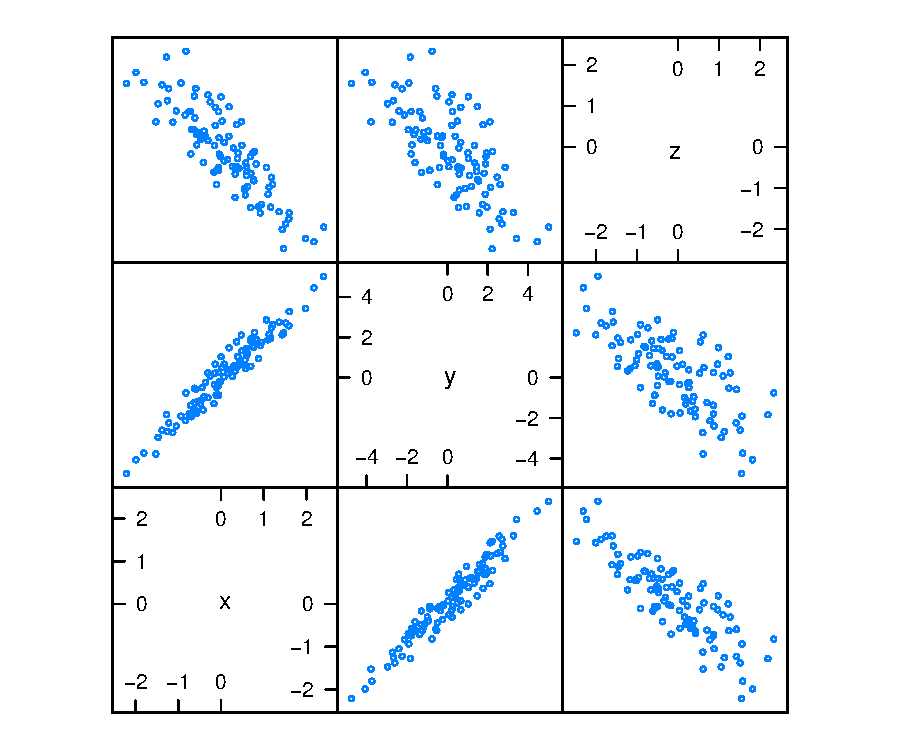
\includegraphics{swv-keepSrc-1-splom}
\caption{100 vectors of random variates ... ...}
\label{fig:AC_Joe}
\end{figure}

\subsection*{Session Information}

\begin{Schunk}
\begin{Sinput}
R> toLatex(sessionInfo())
\end{Sinput}
\begin{itemize}\raggedright
  \item R version 4.0.3 (2020-10-10), \verb|x86_64-pc-linux-gnu|
  \item Locale: \verb|LC_CTYPE=en_US.UTF-8|, \verb|LC_NUMERIC=C|, \verb|LC_TIME=en_US.UTF-8|, \verb|LC_COLLATE=en_US.UTF-8|, \verb|LC_MONETARY=en_US.UTF-8|, \verb|LC_MESSAGES=C|, \verb|LC_PAPER=en_US.UTF-8|, \verb|LC_NAME=C|, \verb|LC_ADDRESS=C|, \verb|LC_TELEPHONE=C|, \verb|LC_MEASUREMENT=en_US.UTF-8|, \verb|LC_IDENTIFICATION=C|
  \item Running under: \verb|Ubuntu 20.04.1 LTS|
  \item Matrix products: default
  \item BLAS/LAPACK: \verb|/usr/lib/x86_64-linux-gnu/openblas-pthread/libopenblasp-r0.3.8.so|
  \item Base packages: base, datasets, graphics, grDevices,
    methods, stats, utils
  \item Other packages: lattice~0.20-41
  \item Loaded via a namespace (and not attached):
    compiler~4.0.3, grid~4.0.3, tools~4.0.3
\end{itemize}\end{Schunk}

\end{document}
